\documentclass{article}
\usepackage{amssymb}
\usepackage[english]{babel}
\usepackage{graphicx}





\begin{document}



\title{Replica and dynamics, similarities and differences.}
\author{Andrea Mazzei }
\maketitle

\begin{abstract}
Aim of this short project is to give an overview of the most important analytical techniques used to deal with mean field spin glasses. The final sections also will present some numerical simulations.
\end{abstract}

\section{Replica approach}\label{prelim}

\subsection{Introduction to replicas}

First of all we need to introduce the replica method, which is a tool used in
the framework of disordered systems to integrate out over the disorder
distribution function. Consider a generic spin system described by a
Hamiltonian that's disorder dependent, and a partition function given by:

\begin{equation}
  Z_J = \sum_{\{S\}} e^{- \beta \mathcal{H}_J}
\end{equation}

where the pedix $J$ describes the disorder dependance. If we want to evaluate
the thermodynamic properties of the system we first have to evaluate the free
energy functional, $- \beta F_J = \log Z_J$, and then perform the average over
the disorder distribution (the so called quenched average). If the evaluation
of $\langle F \rangle_J$ is unaccessible but we can evaluate every moment of
the disorder-integrated partition function $\{Z, Z^2, \ldots, Z^n \}$ we can
obtain $\langle F \rangle_J$ using a known limit.

\begin{equation}
  - \beta \langle F \rangle_J = \langle \log Z_J \rangle = \lim_{n \rightarrow
  0}  \frac{\langle Z_J^n \rangle_J - 1}{n}
\end{equation}

which is the essence of the replica method. When we evaluate $\langle Z^n
\rangle_J$ we are generating $n$ non interacting copies of the system, which
become correlated after averaging over the disorder distribution.

  Replica method (sometimes called replica trick) has been successfully
  applied to a variety of disordered systems, the most notable examples are
  the Sherrington-Kirkpatrick model [Parisi] and to the spherical p-spin model
  [Crisanti & Sommers, Leuzzi].

In this first part we will concentrate on the spherical p-spin model, which is
a RS-1RSB, depending on p, system. Consider the Hamiltonian
\begin{equation}
  \mathcal{H} = \sum_{(i_1 \ldots i_p)} J_{i_1 \ldots i_p} S_{i_1} \ldots
  S_{i_p} - \sum_i h_i S_i
\end{equation}
where each $J$ has been taken by a random distribution and the summation on
$(i_1 \ldots i_p)$ is a sum over each p-uplet of the system.  
The dynamical variables $S_i$ are constrained by $\sum S_i^2 = N$. We will start by describing
shortly the case p = 2.

\subsection{RS 2-spin system}

The Hamiltonial for the 2 spin system is: 

\begin{equation}
  \mathcal{H} = \sum_{(ij)} J_{ij} S_i S_j - \sum_i h_i S_i
\end{equation}

The partition function for replicated system will be the product of each single system partition function.

\begin{equation}
  \langle Z^n \rangle = \sum_{\{S\}^n} e^{- \beta \sum_a^n H [S^a]}
\end{equation}

If we suppose Gaussian distributed disorder we can integrate over its distribution using an Hubbard Stratonovich integration: 

\begin{eqnarray}
  \langle Z^n \rangle &=& \int \prod_{(ij)} d J_{ij} \sum_{\{S\}^n} e^{- \beta \sum_a^n H [S^a] - {{J_{ij}}^2\over {2N}} } \\  
&=&  \sum_{\{S\}^n} e^{(\beta \sum_a \sum_i h_i S_i ^a)} e^{   {   {\beta^2}       \over    {4N^{p-1} }   }  \sum_{i_1\dots i_p}  \sum_{ab} S_{i_1}^a\dots S_{i_p}^a \dots S_{i_1}^b \dots S_{i_p}^b                    }
\end{eqnarray}

The trace over spin states can be evaluated transforming the spherical constraint into its integral representation

\begin{equation}
 \sum_{\{S\}^n} [\dots] = \int \prod_{(ia) }dS_a \delta(\sum_i S_i^2 - N ) [\dots] = \int {d\lambda_a \over \sqrt{2 \pi}}e^{i \lambda_a(\sum_i S_i^2 - N )}  }
\end{equation}

Now we may evaluate the integrals by saddle point methods and obtain the values of $q_{ab}$ and $\lambda_a$.
If we adopt the RS ansatz for this calculation, i.e. $q_{ab} = q*$ and \lambda_a = ?$ we get the RS solution of this model.

By breaking this RS ansatz one should observe that RSB is not present.
This could be either achieved by evaluating the eigenvalues of the free energy's Hessian matrix or noticing that a one-step RSB ansatz would predict the same results of the RS one. This procedure will not be evaluated in the present work, and it will be derived directly in the $p>2$ case.

\subsection{RSB p-spin systems}

If we try the same evaluation scheme for the generic $p > 2$ spin model we have to notice that now the quadratic form in $S$ is missing and is replaced by a p-power term.
So we start by rewriting

DA FINIRE
\begin{equation}
  \langle Z^n \rangle = \int \prod_{(ij)} d J_{ij} \sum_{\{S\}^n} e^{- \beta \sum_a^n H [S^a] - {{J_{ij}}^2\over {2N}} } = \dots
\end{equation}

When we write down the free energy function we see that RS solution is now unstable: this can done both by evaluating the Hessian matrix eigenvalues and going into a one-step RSB ansatz and see if it returns a different solution from the RS one.

\subsection{Direct evaluation}

\subsection{Few words on Ising p-spin}

The framework is very different for the Ising p-spin. It has been shown in literature \ref{isingp} that this model
in zero field presents three different phases. One at high temperatures, where the RS solution is correct and essentially returns the paramagnetic solution. One which appears to be 1 RSB, at intermediate temperatures, and one which is full RSB, just like the Sherrington Kirkpatrick model. 
The 1RSB solution is typical of p-spin systems (with p greater than 2) and seems to be connected with the nonlinearity of associated Langevin equation, that we will describe below.

\section{Dynamic approach}

The dynamic approach is the application of Langevin dynamics to the disordered
spin models. 

\subsection{Few words on Langevin dynamics}

Consider the Hamiltonian discussed before. If we want to implement a dynamic
for the observables $S_i$ we may use the Langevin equation

\begin{equation}
  \frac{dS_i}{dt} = - \frac{\partial \mathcal{H}}{\partial S_i} + \eta_i
\end{equation}

where $\eta$ is a random noise. At this point we have not to confuse $\eta$
with the intrinsic disorder of the system (which is inside the definition of
Hamiltonian). Noise is now delta correlated, i.e. $\bar{\eta} = 0$,
$\overline{\eta_i (t) \eta_j (t')} = 2 T \delta (t - t') \delta_{ij}$. It is
also necessary to distinguish the average over the disorder from the noise
average: the latter will always be performed with an overline, just like the
previous formula.

The noise distribution can be formally written as:

\begin{equation}
P[\eta] = \mathcal{N} e^{-{1\over2}\int dt \int dt' \eta(t) D(t,t') \eta(t')}
\end{equation}

where $D$ is the inverse of the variance of the process.

We can evaluate the average of a generic operator using the integral representation for the Langevin operator

\begin{eqnarray}
\langle O(S) \rangle &=& \int D[\eta] P[\eta] \int D[S] \delta(S - S_\eta) O(S) \\
			&=& 	\int D[S] \delta(S - S_\eta) O(S)\int D[\eta]P[\eta]\delta(\mathcal{L[S]} - \eta)\\
			&=& 	\int D[S] \int D[\hat{S}]  O(S)\int D[\eta]P[\eta] e^{i \int dt \hat{S} [\mathcal{L[S]} - \eta] }
\end{eqnarray}

It is important to remark that the Langevin operator is still disorder- dependent. When averaging over the disorder distribution
the integrals in the previous formula become connected and it becomes possible to write down a new Langevin dynamic with noise $\xi$, where now
$\xi$ is not $\delta$ correlated. A pratical example, with most of calculations omitted, will be presented in the next section.

\subsection{Long time dynamics for the p-spin spherical spin glass}

If we evaluate Langevin dynamic for the spherical p-spin model first of all we can integrate over the spherical constraint, similarly to what we've done in the replica framework.
In these lines we will follow the calculations presented in \cite{CrisantiSommers}. We will skip passages and go straight to the point. 


\begin{equation}
\delta( \sum_i S_i^2 -N) = \int d\mu(t) e^{i\mu ( \sum_i S_i^2 -N) }
\end{equation}

At this point $\mu$ has to be computed in a self-consistent way. 


The dynamic equation now reads

\begin{equation}
  \frac{dS_i}{dt} = - \frac{\partial \mathcal{H}}{\partial S_i} - \mu (t) S_i + \eta_i
\end{equation}

After a bit of calculation we can get the time evolution equation for the correlation function

\begin{equation}
EQTN MISSING

LOTS OF EQTNS MISSING
\end{equation}

When combining this equation with the criterion that $C$ is time-decreasing at any given time, we get that
the inequality cannot hold if the temperature is lower than $T_d$, with 

\begin{equation}
T_d = \sqrt{  {p(p-2)^{p-2}}      \over      {2(p-1)^{p-1}}} 
\end{equation}

which is always higher than the static temperature mentioned in the replica approach.
 The meaning of this picture is that at a temperature in the $T_d$ neighborhood, 
metastable states (thus not weighing in the static measure) dominate the dynamic of the system.
 In this sense, the $T_d$ transition is purely dynamical.

At this point an observation is important. Both the dynamical temperature and the static one are,
 in the 2-spin spherical mean field spin glass, equal to zero.


\section{Similarities and differences}

So far we have described two methods used to approach to the study of a
disordered system. One is static, its aim is to find the thermodynamic of the
systems by explicitely evaluating the average over the Boltzmann measure and
the disorder distribution. The informations on eventual transitions and other
critical phenomena are encoded in the usual thermodynamic functions, such as
entropy and free energy. The other is dynamical, meaning that we are searching
for transitions and other critical phenomena observing the time evolution of
specific correlation functions.

In the high temperature phases the two methods coincide. 
In the low temperature phase both present
interesting issues and phenomena, which essentially decode some aspects of the same complex behaviour, 
though very important differences begin to arise.

First of all, the dynamic approach identifies a $T_d$ temperature at which ergodicity is broken, whilst the replica approach identifies a single paramagnetic stable state, which seems to underline that ergodicity is not broken in the $T>T_s$ regime. Moreover, the replica approach does not identifies any $T_d$.

The second issue is that the dynamical approach is not able to investigate the properties of the system in the aging regime.The natural question emerging now is: which of the two methods is correct? The answer is that both methods are correct in a specific regime ( The replicas in the $T<T_s$ and $T>T_d$, whilst approaching the $T_d$ they are not able to recover the long time dynamics and aging properties. The dynamic appoach gives correct results in the surroundings of $T_d$, predicting slow dynamics and aging properties. Nonetheless , dynamic approach gives inconsistent results in the very-low-$T$ phase).


\begin{figure}[h]
		\includegraphics{img_repvsdyn.png}
	\label{fig:img_multispin}
	\caption{Multispin Coding: 3 sites have R replicas, all of them are updated using a single bitwise operation}

\end{figure}



\section{RSB and Ergodicity breaking in simulations}

In the next section I will present some numerical simulations on the Ising p-spin system. 
The choice of a different spin system is purely for sake of simplicity in the simulation.
If we'd want to simulate a system with the spherical constraint (which is of course a continous system)
we'd have to take into account some additional problematics: 

\begin{itemize}
\item {implement a dynamic which preserves the constraint}

Our Montecarlo simulation will have to satisfy the constraint for each move. This can be done in two ways: 
either by satisfying the constraint at each move or by implement a soft spin version which has our original
constraint as a limit. 
The first method must of course update at least two spins (or more) simultaneously, and I was not sure about
nor the details of convergence of the algorithm nor the satisfiability of detailed balancing, even though it seems that this method was already been investigated
in literature.
The second method is indeed easier to implement. It could be a choice but it still soffers two issues described below 
these lines.

\item {Mean field systems require more memory and much more operations}

A connectivity tensor of a system with $N$ sites requires an $N \cross N \cross \dots N$ matrix with inside the information
on the quenched disorder. If we insted consider a random graph with $Z$ neighbors per site, 
we could store the same information in two matrices $N \cross (Z-1)P$, name it $C$ and $J$, where $C$ remembers 
the label of each neighbor present in the p-uplet and each p-uplet, and $J$ has inside the numerical value o
of the disorder.

Furthermore, any update in mean field requires the evaluation of, and some operations 
on, a large number of spins. This would severely slow down the code.

\item {Continous dynamic require a double arithmetic}

A bool arithmetic is much more efficient than a double one. 

\end{itemize}


\subsection{Few words on multispin coding}

Multispin coding is a coding technique implemented to run fast simulations on
Ising spins. Since an ising spin is essentially a boolean variable, we are
allowed to imagine that a long integer variable (32 bits), when expressed in
bit representation, contains informations on 32 spins. If we have $N$ long
int, we can imagine that we have informations on 32 systems of $N$ sites each.

The interesting thing is that if we can write the Hamiltonian using bitwise
operations, instead of using integer (or worse, floating point) algebra, we
will have two great advantages: First is that bitwise operations are pretty
fast by itselves, so we will gain some computation time in this operation.
Second, and more important, is that we can evolve 32 spins using a single
operation! Of course, we may have to multiply the result of a bitwise
operation with a floating point number, so that the algebra is essentially
floating point. But the crucial operations of the simulations are still
boosted.


\begin{figure}[h]
		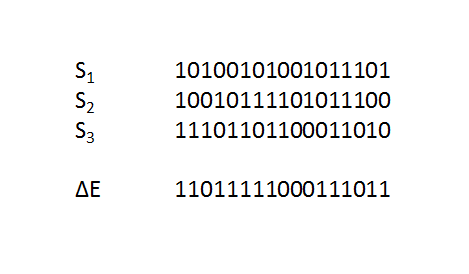
\includegraphics{img_multispin.png}
	\label{fig:img_multispin}
	\caption{Multispin Coding: 3 sites have R replicas, all of them are updated using a single bitwise operation}

\end{figure}

As example, the definition of Hamiltonian is given for a 3-spin Ising model:
\begin{equation}
  \mathcal{H} (S_1, S 2, S_3) = A (S_1 \oplus S_2 \oplus S_3) + B
\end{equation}
where the $\oplus$ sign represents the bitwise XOR operation.


\subsection{Dynamic arrest in simulations}

In this section i will present some simulation on Ising p-spin and show that
dynamic arrest occurs, similarly to what happens in the Dynamical framework
presented before. If we save from simulations the time evolution of the overlap matrix, we can see that, 
in the high temperature phase all the overlaps fastly decrease to zero, but if we are approaching low 
temperatures those seem to stuck to nonzero values.


\begin{figure}[h]
		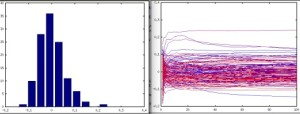
\includegraphics{metro2.jpg}

\label{fig:img_e}
	\caption{Comparison in slowing down on the time series: A metropolis simulation showing dynamical arrest  in the region $\beta = 1$. 
	Time in the x axis is scaled on sampling time,  $N^4 / 100$}

\end{figure}

This is indeed a method to roughly determine via-simulations the eventual presence of dynamical arrest, even though I
found some difficulties in the evaluation of the exact $T_d$. 

\subsection{Tempering}

By looking the relaxation curves for the replica overlaps of the system, we can see that below the dynamical temperature dynamic arrest occurs. That is, the overlap values do not go to zero, while the equilibrium properties at this temperature suggest us that the overlap distribution should be $P(Q) = \delta(Q-0)$.


However, there is a possible workaround to estimate the correct overlap distribution at equilibrium, and is given by parallel tempering. 

Parallel tempering is a  technique for simulation boosting invented to deal with problems involving multi-basin sampling.
The idea is to evolve a certain number of 'replicas' (technically these are not replicas of the system, since they are at higher temperatures) at temperatures higher that the sampling ones.
HIgher temperatures allows those probes to sample the energy landscape without being freezed in a single basin.
When a high temperature probe finds a basin that has similar energy to the real system, the simulation allows the exchange of temperatures, letting the cold probe to sample the new basin, and turning the old sampler into an high temperature probe. By means of this implementation, parallel tempering is usually also referred as replica exchange method.

\begin{figure}[h]
		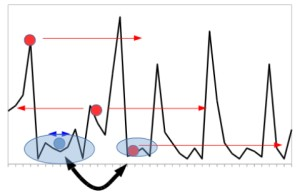
\includegraphics{imgtemper3.jpg}
	\label{fig:imgtempering}
	\caption{Parallel tempering allows sampling in different basins, thus preventing the effects of critical slowing down}
\end{figure}

The detail of the algorithm is very similar to the one used in the Metropolis algorithm. When a certain number of Montecarlo sweeps have been made on the system, replica exchange picks two configurations at random, $\{S_a,\beta_a\},\{S_b,\beta_b\}$, and evaluates the probability of the move, according to Metropolis Hastings algorithm. 

\begin{equation}
p = \min ( 1, { \exp( -\beta_a E[S_b] - \beta_b E[S_a]) \over \exp( -\beta_a E[S_a] - \beta_b E[S_b])   } )
\end{equation}

The ratio of the two exponential may be re-evaluated with some simple algebra to obtain

\begin{equation}
p = \min ( 1, { \exp(  \Delta \beta \Delta E   } ) 
\end{equation}

It is easy to see that this condition satisfies detailed balance.

\begin{figure}[h]
		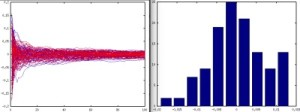
\includegraphics{temp2.jpg}
		\label{fig:img_e}
	\caption{Comparison in slowing down on the time series: A parallel tempering in the region $\beta = 1$. We can see a very different picture if we compare this with the preceding one
	Time in the x axis is scaled on sampling time,  $N^4 / 100$}
\end{figure}

In this way we should be able to recover the static properties of the system under the condition of dynamical arrest.
As we can see from pictures, at low but not extreme temperatures, the system is now able to relax around the correct overlap distribution, which is $P(Q) = \delta(Q)$. 







{\newpage}

{\newpage}




\begin{thebibliography}{99}

  {\bibitem{CrisantiSommers}A. Crisanti, H.J. Sommers, {\tmem{The spherical p-spin interaction spin-glass model, Dynamics }}, Z. Phys. B 92, 25%271 (1993) }


  {\bibitem{Crisanti2}A. Crisanti, L. Leuzzi, {\tmem{The spherical p-spin interaction spin-glass model, Static}},  Z.Phys.B Condensed Matter 87, 341-354 (1992) )}


  {\bibitem{Parisi}G. Parisi, {\tmem{Title}}, Journal/Editor, (year)}


  {\bibitem{Kosterlitz}}Kosterlitz, {\tmem{Title}}, Journal/Editor, (year)}


  {\bibitem{Pedestrians}C. Castellani, A. Cavagna, {\tmem{Spin glass theory for pedestrians}}}

   {\bibitem{isingp} V. M. de Oliveira, J.F. Fontanari {\tmem{Replica analysis of the p-spin interactiFon Ising spin-glass model }},J. Phys. A Volume 32, Number 12)}

\end{thebibliography}


















\end{document}
